\section{Introduction}

\begin{frame}{Problem statement}

Development of a control scheme in case of \textbf{rotor failure}, to allow the quadrotor to land with only three actuators.

\end{frame}

\begin{frame}{Proposed Strategy}

\textbf{Full control of attitude is lost}: renounce the yaw angle control, maintaining flight control of a spinning vehicle\\
\bigskip
\textbf{Double-loop architecture}\\
\begin{list}{$ \circ $}{}
	\item \textit{Outer Control}\\
	Yaw velocity is computed instead of the yaw angle\\
	\bigskip
	\item \textit{Inner Control}\\
	Roll angle, pitch angle and yaw velocity regulated via feedback linearization
\end{list}

\end{frame}

\section{Quadrotor Model}

\begin{frame}{Control Model}

\begin{columns}
\begin{column}{0.3\textwidth}
\begin{itemize}
	\item Symmetric
	\bigskip
	\item Rigid propellers
	\bigskip
	\item Linear drag
\end{itemize}
\end{column}
\begin{column}{0.7\textwidth}
\begin{figure}
	\centering
	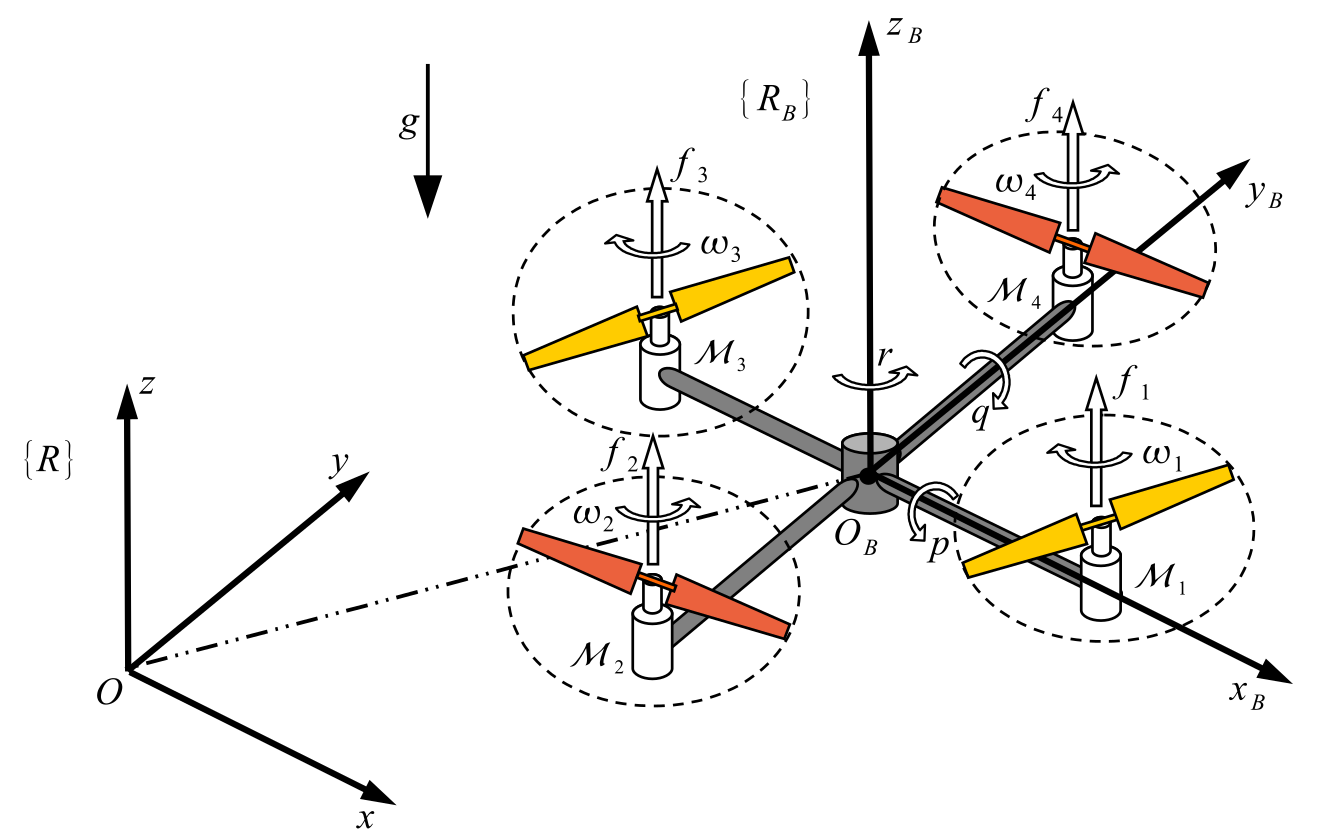
\includegraphics[width=0.9\linewidth]{Images/Quad_model}
\end{figure}
\end{column}
\end{columns}
Two reference frames:\\
\bigskip
\begin{itemize}
\item Earth frame: $ \{R\}\{O, x, y, z\} $
\item Body-fixed frame: $ \{R_b\}\{O_b, x_b, y_b, z_b\} $
\end{itemize}

\end{frame}

\begin{frame}{Control Model}

\textbf{Rotations} along roll ($ \phi $) and pitch ($ \theta $) angles are constrained:
\begin{equation*}
(-\frac{\Pi}{2}<\phi<\frac{\Pi}{2}), \qquad (-\frac{\Pi}{2}<\theta<\frac{\Pi}{2})
\end{equation*}
while yaw angle $ \psi $ is unconstrained.\\
\bigskip
\textbf{Inertia matrix} in the body frame:
\begin{equation*}
\mathbf{I}=
\begin{bmatrix}
I_{xx} & 0 & 0 \\
0 & I_{yy} & 0 \\
0 & 0 & I_{zz} 
\end{bmatrix}
\end{equation*}
where $ I_{xx} = I_{yy} $ due to symmetry.

\end{frame}

\begin{frame}{Control Model}

\textbf{Dynamic model}, defined from generalized forces, drag force and weight:
\begin{equation*}
\begin{cases}
\ddot{x} = \frac{1}{m}[(C_{\phi}S_{\theta}C_{\psi} + S_{\phi}S_{\psi})u_f-k_t \dot{x}] \\
\ddot{y} = \frac{1}{m}[(C_{\phi}S_{\theta}S_{\psi} - S_{\phi}C_{\psi})u_f-k_t \dot{y}] \\
\ddot{z} = \frac{1}{m}[(C_{\phi}C_{\theta})u_f- mg - k_t \dot{z}] \\
\dot{p} = \frac{1}{I_{xx}}[-k_r p - qr(I_{zz}-I_{yy})+\tau_p]  \\
\dot{q} = \frac{1}{I_{yy}}[-k_r q - pr(I_{xx}-I_{zz})+\tau_q]  \\
\dot{r} = \frac{1}{I_{zz}}[-k_r r - pq(I_{yy}-I_{xx})+\tau_r]  \\
\dot{\phi} = p + q S_{\phi}T_{\theta} + r C_{\phi}T_{\theta} \\
\dot{\theta} = q C_{\phi} - rS_{\phi} \\
\dot{\psi} = \frac{1}{C_{\theta}}[qS_{\phi}+rC_{\phi}]
\end{cases}
\end{equation*}

\begin{itemize}
\item $ k_r, k_t $ = rotational and linear drags, $ N \cdot m \cdot s  $;
\item $ u_f $ = total upward lift force, $ N $;
\item $ \tau_p, \ \tau_q, \ \tau_r $ = torque around roll, pitch and yaw axis, $ N\cdot m $;
\end{itemize}

\end{frame}

\begin{frame}{Control Model}
\textbf{System inputs}:\\ Generalized forces $ u_f, \ \tau_p, \ \tau_q, \ \tau_r $\\
\bigskip 
\textbf{Real actuation}:\\
Four motors forces $ f_1, \ f_2, \ f_3, \ f_4 $\\
\bigskip
Relation between these is given by:
\begin{equation}
\begin{bmatrix}
u_f \\ \tau_p \\ \tau_q \\ \tau_r
\end{bmatrix} = 
\begin{bmatrix}
1 & 1 & 1 & 1 \\
0 & -l & 0 & l \\
-l & 0 & l & 0 \\
d & -d & d & -d
\end{bmatrix}
\begin{bmatrix}
f_1 \\ f_2 \\ f_3 \\ f_4
\end{bmatrix}
\label{force_mapping}
\end{equation}
where
\begin{itemize}
\item \textit{d} = ration between drag and thrust coefficient of the rotor, $ m $
\item \textit{l} = arm length, $ m $
\end{itemize}

\end{frame}